% ОБЯЗАТЕЛЬНО ИМЕННО ТАКОЙ documentclass!
% (Основной кегль = 14pt, поэтому необходим extsizes)
% Формат, разумеется, А4
% article потому что стандарт не подразумевает разделов
% Глава = section, Параграф = subsection
% (понятия "глава" и "параграф" из документа, описывающего диплом)
\documentclass[a4paper,article,14pt]{extarticle}

% Подключаем главный пакет со всем необходимым
\usepackage{spbudiploma_tempora}

% Пакеты по желанию (самые распространенные)
% Хитрые мат. символы
\usepackage{euscript}
% Таблицы
\usepackage{longtable}
\usepackage{makecell}
% Картинки (можно встявлять даже pdf)
\usepackage[pdftex]{graphicx}

\usepackage{amsthm,amssymb, amsmath}
\usepackage{textcomp}
\usepackage[newfloat]{minted}
\usepackage{biblatex}
\addbibresource{refs.bib}

\usepackage{xurl} % Fix weird links in bibliography

\newenvironment{code}{\captionsetup{type=listing}}{}
\SetupFloatingEnvironment{listing}{name=Исходный код}

\begin{document}

% Титульник в файле titlepage.tex
% --------------------- Титульник ВКР СПбГУ -----------------------------
% Автор: Тоскин Николай, itonik@me.com
% Если заметили ошибку, напишите на email
% Если хотите добавить изменение самостоятельно:
% https://github.com/itonik/spbu_diploma/
% Использованы материалы:
% habr.com/ru/post/144648/
% cpsconf.ru
% Документы ниже могут уже быть неактуальны, тем не менее за годы ничего
% нового не появилось
% Текст:
% http://edu.spbu.ru/images/data/normativ_acts/local/20181030_10432_1.pdf
% Титульный лист:
% http://edu.spbu.ru/images/data/normativ_acts/local/20180703_6616_1.pdf
% -----------------------------------------------------------------------

% Титульный лист диплома СПбГУ
% Временное удаление foot на titlepage
\newgeometry{left=30mm, top=20mm, right=15mm, bottom=20mm, nohead, nofoot}
\begin{titlepage}
\begin{center}

\textbf{Санкт--Петербургский}
\textbf{государственный университет}

\vspace{35mm}

\textbf{\textit{\large ЦАРЁВ Никита Евгеньевич}} \\[8mm]
% Название
\textbf{\large Выпускная квалификационная работа}\\[3mm]
\textbf{\textit{\large Разработка обучающего веб-инструмента удаленной сборки и интерактивной отладки программ}}

\vspace{20mm}
Уровень образования: бакалавриат\\
Направление 01.03.02 «Прикладная математика и информатика»\\
Основная образовательная программа СВ.5005.2018
«Прикладная математика, фундаментальная информатика и программирование»\\
Профиль «Современное программирование»\\[15mm]


% Научный руководитель, рецензент
\begin{flushright}
\begin{minipage}[t]{0.65\textwidth}
{Научный руководитель:} \\
профессор, факультет математики и компьютерных наук Санкт--Петербургского
государственного университета, д.ф. - м.н. Куликов~Александр Сергеевич

\vspace{10mm}

{Рецензент:} \\
доцент Новгородского государственного университета имени Ярослава Мудрого,
к. т. н. Довгалюк~Павел Михайлович
\end{minipage}
\end{flushright}

\vfill

{Санкт-Петербург}
\par{\the\year{} г.}
\end{center}
\end{titlepage}
% Возвращаем настройки geometry обратно (то, что объявлено в преамбуле)
\restoregeometry
% Добавляем 1 к счетчику страниц ПОСЛЕ titlepage, чтобы исключить
% влияние titlepage environment
\addtocounter{page}{1}


% Содержание
\tableofcontents
\pagebreak

\specialsection{Введение}

В настоящее время обучение языку ассемблера является важной составляющей многих программистских курсов.

Очень часто студенты, изучающие язык ассемблера, сталкиваются с проблемами при настройки среды разработки, при использовании инструментов компиляции и отладки.

Преподаватели таких курсов также сталкиваются с проблемами организации учебного процесса.

Создание удобного, интерактивного и производительного программного инструмента удалённой сборки и отладки програм на ассемблере, представляет собой актуальную задачу.

\specialsection{Постановка задачи}

\textbf{Цель данной работы} состоит в разработке обучающего веб-инструмента удалённого запуска, отладки и проверки программ на языке ассемблера.

\textbf{Задачи данной работы}:

\begin{enumerate}
    \item Исследование существующих решений для запуска и отладки программ на языке ассемблера, а также решений для обучения языку ассемблера.
    \item Формирование требований к разрабатываемому инструменту.
    \item Исследование возможности создания инструмента.
    \item Разработка программной архитектуры инструмента.
    \item Реализация инструмента.
    \item Исследование свойств решения.
\end{enumerate}

\textbf{Объектом исследования} являются системы запуска и отладки программ на языке ассемблера.

\textbf{Предметом исследования} является наглядность и удобство использования таких систем в учебном процессе.

\textbf{Практическая ценность работы} состоит в том, что разработанный инструмент позволит проводить обучение языку ассемблера более эффективно для студентов.

\pagebreak
\section{Обзор предметной области}
\subsection{Критерии сравнения и отбора аналогов}

В мире существует множество решений для запуска ассемблерного кода, а также решений для обучения языку ассемблера. В этой главе рассматривается несколько таких решений, каждое из них анализируется в контексте следующих \textbf{критериев сравнения}:

\begin{enumerate}
    \item Поддержка запуска ассемблерного кода на разных диалектах и на разных архитектурах.
    \item Поддержка отладки: выполнение по шагам, поддержка точек останова, редактирования регистров/памяти, визуализация стека вызовов.
    \item Поддержка задач и их автоматической проверки.
    \item Поддержка интеграции с системами управления обучением.
    \item Возможность работы без установки дополнительного программного обеспечения на устройстве пользователя.
    \item Возможность самостоятельной установки и развёртывания системы на выделенном сервере, доступность исходного кода.
\end{enumerate}

Альтернативные решения искались по запросам ``online assembly debugger'', ``online assembly ide'', ``educational assembly ide''. Также были рассмотрены популярные решения для организации учебного процесса при использовании других языков программирования.

\subsection{Существующие решения}
\subsubsection{Ideone}

Ideone\cite{ideone} является онлайн компилятором и средой разработки, поддерживающей более 60 языков программирования, в том числе несколько диалектов ассемблера.

Поддерживается запуск ассемблерного кода на архитектурах x86 (Intel и AT\&T диалекты) и x86-64 (только Intel диалект). Отладка не поддерживается. Поддержки задач, их автоматической проверки нет, соответственно нет и интеграции в системы управления обучением.

Взаимодействие с системой происходит через веб-интерфейс, установки допольнительного ПО не требуется. Система имеет закрытый исходный код, самостоятельно установить систему на выделенный сервер не представляется возможным.

\subsubsection{OneCompiler}

OneCompiler\cite{onecompiler} является онлайн компилятором и средой разработки, поддерживающей, в том числе, и Intel диалект x86 ассемблера.

Поддержиывается запуск кода, есть возможность указать содержимое стандартного потока ввода перед запуском. Отладка не поддерживается. Поддержки задач, их автоматической проверки нет, соответственно нет и интеграции в системы управления обучением.

Взаимодействие с системой происходит через веб-интерфейс, установки допольнительного ПО не требуется. Система имеет закрытый исходный код, самостоятельно установить систему на выделенный сервер не представляется возможным.

\subsubsection{ASM Debugger}

ASM Debugger\cite{asmdebugger} является инструментом для пошаговой отладки простых программ на языке ассемблера. Особенностью инструмента является то, что он не использует запуск программ на реальном аппаратном обеспечении. Вместо этого, на языке Javascript реализовано подмножество инструкций x86 ассемблера.

Поддерживается запуск ассемблерного кода на архитектуре x86 с Intel диалектом. Поддерживается пошаговое исполнение, просмотр значений регистров. Поддержки задач, их автоматической проверки нет, соответственно нет и интеграции в системы управления обучением.

Взаимодействие с инструменетом происходит через веб-интерфейс, установки допольнительного ПО не требуется. Инструмент имеет открытый исходный код, установки серверной части не требуется, так как вся логика инструмента исполняется в браузере клиента.

\subsubsection{Davis}

Davis\cite{davis} является инструментом для запуска и пошагового исполнения простых программ на языке ассемблера. Как и ASM Debugger, данный инструмент включает в себя реализацию эмулятора x86 ассемблера, использующего диалект Intel. Эмулятор написан на языке TypeScript и реализует основные арифметические инструкции, условные и безусловные переходы, инструкции работы со стеком. Также поддерживается инструкция INT, позволяющая выполнять вывод на экран.

Инструмент предоставляет возможность пошагового исполнения, установки точек останова, просмотра содержимого регистров и памяти. Можно настроить частоту исполнения инструкций в режиме исполнения: от 100 до 500 миллисекунд.

Поддержки задач, их автоматической проверки и интеграции в системы управления обучением нет. Также как и ASM Debugger, данный инструмент доступен через веб-интерфейс, причём серверная часть отсутствует. Инструмент имеет открытый исходный код.

\subsubsection{OnlineGDB}

OnlineGDB\cite{onlinegdb} является онлайн компилятором, отладчиком и средой программирования, поддерживающим более 20 различных языков программирования. Для многих из них, например для C, C++ и языка ассемблера, поддерживается интерактивная отладка. При работе с этими языками создаётся интерактивная сессия в отладчике GDB.

Поддерживается запуск ассемблерных программ на архитектуре x86-64 с AT\&T диалектом. Программе можно передать аргументы командной строки, а также взаимодействовать с ней через стандартные потоки ввода и вывода. Поддерживается запуск в режиме отладки, позволяющий устанавливать точки останова, просматривать информацию о состоянии регистров, стека вызовов, а также следить за произвольными выражениями. Инструмент позволяет исполнять программу по шагам, до выхода из функции, или до следующей точки останова. Также можно выполнять произвольные команды отладчика GDB.

Существует поддержка создания учебных классов из веб-интерфейса. В них можно добавлять преподавателей и студентов, а также публиковать задания. В заданиях можно задавать режим проверки: ручной или автоматический. В автоматическом режиме проверки программа запускается на наборе тестов. Каждый тест представляет из себя входные данные и эталонный ответ. При запуске программы, входные данные записываются ей на стандартный поток ввода, а вывод программы сравнивается с эталонным ответом. Также для задания можно указать шаблон кода, который будет показан студенту вместо пустого окна редактора перед выполнением работы. Интеграции с существующими системами управления обучением нет, но существует возможность просмотра результатов выполнения задания в виде таблицы.

Инструмент имеет закрытый исходный код, установка его на выделенный сервер не представляется возможным.

\subsubsection{SASM}

SASM\cite{sasm} представляет из себя кроссплатформенную среду разработки на языке ассемблера для архитектур x86 и x86-64 с использованием ассемблеров NASM, GNU Assembler, FASM, MASM. Поддерживаются диалаекты Intel и AT\&T.

Поддерживается запуск ассемблерного кода, поддерживается выполнение по шагам, точки останова, просмотр и редактирование регистров и памяти, а также произвольные команды GDB.

Поддержки задач, их автоматической проверки нет, соответственно нет и интеграции в системы управления обучением.

Для использования инструмента необходима его установка на компьютер пользователя. Инструмент имеет открытый исходный код.

\subsubsection{JetBrains Clion + EduTools}

Clion\cite{clion}~--- это интегрированная среда разработки от компании JetBrains, предназначенная, в первую очередь, для разработки приложений на языках C и C++. Язык ассемблера не поддерживается ни в каком виде, но существуют сторонние плагины, которые решают эту проблему, например NASM Assembly Language\cite{nasmplugin}.

Компиляция и запуск кода на языке ассемблера возможны, если модифицировать должным образом файлы системы описания сборки CMake. Отладка ассемблерного кода не поддерживается.

Плагин EduTools\cite{edutools} позволяет создавать и писать задачи с автоматическими тестами, что упрощает проверку решений. Отсутствует поддержка задач с закрытыми (недоступными для обучающегося) тестами. Интеграция с системами управления обучением отсутствует.

Для использования данной среды разработки необходима её установка на компьютер пользователя. Она имеет закрытый исходный код.

\subsubsection{GitHub Classroom + Visual Studio Code}

GitHub Classroom\cite{githubclassroom}~--- это сервис, позволяющий давать учебные задания в виде git-репозиториев. GitHub Classroom предоставляет возможность добавить кнопку <<открыть в Visual Studio Code>>\cite{githubclassroomvscode}, которая позволяет открыть репозиторий с преднастроенными плагинами в этом редакторе.

Для того, чтобы настроить поддержку языка ассемблера в Visual Studio Code, требуется установка дополнительных плагинов. Также преподавателю в шаблонном репозитории необходимо будет настроить компиляцию и запуск в файлах \texttt{tasks.json} и \texttt{launch.json}. Отладка не поддерживается.

GitHub Classroom позволяет добавлять тесты через веб-интерфейс преподавателя. В качестве теста может выступать набор входных данных и эталонных ответов к ним, так и путь до скрипта для автоматической проверки. В первом случае входные данные передаются программе через стандартный поток ввода, а вывод программы сравнивается с эталонным ответом.

На компьютер пользователя необходимо устанавливать Visual Studio Code, компилятор и отладчик. GitHub Classroom имеет закрытый исходный код, установить свою копию на выделенный сервер не представляется возможным.

\subsubsection{Stepik}

В системе управления обучением Stepik\cite{stepik} есть режим задания Code Challenge, который позволяет проверять код, написанный на различных языках программирования. Поддерживается Intel диалект x86 и x86-64 ассемблера. Отладка запускаемого кода не поддерживается.

Поддерживаются задачи и их автоматическая проверка на скрытых тестах. Тесты должны иметь вид набора входных данных и эталонных ответов. Входные данные передаются программе через стандартный поток ввода, а вывод программы сравнивается с эталонным ответом. Взаимодействие с системой происходит через веб-интерфейс, установка дополнительного ПО не требуется. Система имеет закрытый исходный код.

\subsubsection{Moodle + Virtual Programming Lab}

Для системы управления обучением Moodle\cite{moodle} существует плагин Virtual Programming Lab\cite{vpl}, котторый позволяет запускать и проверять код, написанный на различных языках программирования.

Поддерживается Intel диалект x86 ассемблера, отладка не поддерживается. Поддерживаются задачи и их автоматическая проверка на скрытых тестах. Тесты должны иметь вид набора входных данных и эталонных ответов. Входные данные передаются программе через стандартный поток ввода, а вывод программы сравнивается с эталонным ответом.

Взаимодействие с системой происходит через веб-интерфейс, установка дополнительного ПО не требуется. И система Moodle и плагин Virtual Programming Lab имеют открытый исходный код. Соответственно, есть возможность установки этой связки на выделенный сервер.

\subsubsection{Git репозиторий с заданиями и скриптами для проверки}

Одним из популярных способов организовать проверку заданий при проведении курсов по программированию является специально организованный git репозиторий. К примеру может ожидаться, что студенты выполняют задания в своих локальных копиях, а задания проверяются специально написанными скриптами, расположенными в том же репозитории.

При таком подходе, учащиеся могут выбирать любой удобный им редактор кода. Для запуска кода могут быть предоставлены готовые скрипты. То же самое нельзя сказать об отладке, скорее всего студенту придётся познакомиться с GDB или другой подобной утилитой.

Такой подход применяется в учебном процессе на практике. Возможно автоматизировать и генерацию репозиториев с задачами для каждого пользователя, и закрытые тесты, и даже интеграцию с системами управления обучением. На практике таким мало кто занимается.

Такой подход требует от орагнизаторов курса реализовать скрипты запуска и проверки решений. От студентов же требуется установка дополнительного программного обеспечения (такого как git, компилятор, отладчик) и наличие навыков работы с инструментами командной строки. Также может требоваться использование конкретной операционной системы, так как зачастую скрипты расчитывают на наличие конкретного пользовательского окружения.


\subsection{Сравнение существующих решений}

Краткая информация о решениях представлена в таблице \ref{table:alternatives}.

\begin{center}
\small
    \begin{longtable}{|p{3.5cm}|p{2cm}|p{2cm}|p{2cm}|p{2cm}|p{2cm}|}
    \caption{Сравнение существующих решений}\label{table:alternatives} \\
    \hline
    \textbf{Решение} & \textbf{Диалект} & \textbf{Отладка} & \textbf{Учебный процесс} & \textbf{Нужна установка} & \textbf{Открытый исходный код} \\
    \hline
    Ideone & x86 (Intel, AT\&T), x86-64 (Intel) & нет & нет & нет & нет \\ \hline
    OneCompiler & x86 Intel & нет & нет & нет & нет \\ \hline
    ASM Debugger & x86 Intel (подмножество) & да\footnote{Поддерживается пошаговое исполнение, просмотр значений регистров} & нет & нет & да \\ \hline
    Davis & x86 Intel (подмножество) & да\footnote{Поддерживается пошаговое исполнение, просмотр значений регистров и памяти} & нет & нет & да \\ \hline
    OnlineGDB & x86-64 AT\&T & да & да & нет & нет \\ \hline
    SASM & x86, x86-64 (Intel, AT\&T) & да & нет & да & да \\ \hline
    Clion + EduTools & x86 Intel\footnote{Только со сторонним плагином} & нет & частично\footnote{Задачи поддерживаются, интеграции с системами управления обучением нет} & да & нет \\ \hline
    GitHub + VSCode & зависит от настроек & нет & частично & да & нет \\ \hline
    Stepik & x86, x86-64 Intel & нет & да & нет & нет \\ \hline
    Moodle + VPL & x86 Intel & нет & да & нет & да \\ \hline
    Git репозиторий & зависит & нет & частично & да & --- \\ \hline
    \end{longtable}
\normalsize
\end{center}

Среди расмотренных альтернатив можно выделить несколько групп схожих решений.

Первой такой группой являются онлайн компиляторы. К ним можно отнести Ideone и OneCompiler. Они представляют веб редакторы с возможностью компиляции и запуска кода на разных языках. В этих системах языку ассемблера не уделяется особого внимания, так как основная масса пользователей таких систем использует их для написания кода на высокоуровневых языках. Также эти системы имеют закрытый исходный код.

В качестве второй группы можно выделить такие системы как Stepik, Moodle и JetBrains EduTools. Они предназначены, в первую очередь, для образовательных процессов. Поддержка задач, направленных на иизучение языка ассемблера, не является их основной целью. Так, для системы Moodle, требуется сторонний плагин, а среды разработки JetBrains поддерживают механизм отладки многих языков программирования, но не ассемблера.

В качестве ещё одной группы решений можно выделить ASM Debugger и Davis. Они представляют из себя простые веб-инструменты для запуска и пошагового исполнения ассемблерного кода. Эти инструменты реализуют подмножество инструкций x86 ассемблера и исполняются не на реальном процессоре, а напрямую в браузере пользователя. Помимо отсутствия поддержки запуска на настоящих машинах, у этих инструментов есть ещё и другой недостаток: отсутствие возможности интеграции в процесс обучения из-за того, что они исполняются исключительно на стороне пользователя.

Также хочется выделить решения, требующие сложной настройки со стороны преподавателей, такие как интеграция GitHub Classroom с Visual Studio Code и использование git репозитория для организации учебного процесса. Эти решения отличаются гибкостью, но требуют написания скриптов и конфигурационных файлов перед использованием. Также они требуют установки дополнительного программного обеспечения на компьютерах студентов.

В качестве последней группы можно рассмотреть такие инструменты, как SASM и OnlineGDB. Они имеют полную поддержку запуска и отладки ассемблерного кода, и используют настоящие компиляторы и отладчики для этого. OnlineGDB также отличается другими выгодными свойствами: он работает через веб-интерфейс, а также предоставляет определённые возможности для создания учебных комнат, заданий и их автоматической проверки. К сожалению, этот инструмент обладает и недостатками: отсутствие возможности установить серверную часть на выделенный сервер из-за закрытогоо исходного кода. Также, несмотря на возможность создания заданий для студентов, в обоих этих инструментах отсутствует интеграция с другими системами управления обучением, что означает необходимость синхронизировать данные о пользователях и оценках между этими системами вручную.

\subsection{Выводы}

В этой главе были рассмотрены различные решения для запуска и отладки программ на языке ассемблера, а также решения, предназначенные для обучения языку ассемблера. Все рассмотренные решения по умолчанию работают только с архитектурами x86/x86-64. Во всех рассмотренных инструментах не хватает какой-либо важной функциональности. Большинство инструментов, имеющих функционал отладки ассемблерного кода, не поддерживают интеграцию в учебный процесс, а системы управления обучением не поддерживают отладку ассемблерного кода. Некоторые решения требуют явной установки на компьютер пользователя, что влечёт за собой проблемы с совместимостью и удобством использования. Также можно отметить, что значительная часть рассмотренных альтернатив являются проприетарными решениями. В частности, нельзя гарантировать доступность проприетарных веб-инструментов в течение длительного времени.

\pagebreak
\section{Формулировка требований к решению}

Наиболее важными характеристиками разрабатываемого инструмента будут те, которые выгодно его отличают от существующих аналогов. Исходя из этого, были сформулированы следующие функциональные требования к инструменту:

\begin{enumerate}
    \item Инструмент должен быть доступен через веб-интерфейс и не требовать установки допольнительного программного обеспечения на устройстве пользователя.
    \item Инструмент должен содержать возможность аутентификации пользователей по протоколу LTI, а учащиеся должны уметь получать задания по конкретным задачам через системы управления обучением.
    \item На странице задания для учащегося должно быть доступно условие задачи, редактор кода, возможность отправить решение на проверку и информация о предыдущих попытках решения.
    \item Вместе с редактором кода должна быть доступна функциональность отладки: добавление и удаление точек останова, запуск, остановка, пошаговое исполнение программы, должен быть доступен просмотр и редактирование регистров процессора, а также вычисление произвольных выражений.
    \item Запускаемые пользовательские программы должны быть ограничены по времени и используемой памяти, им должен быть запрещен доступ к файловой системе, сети, процессам и другим ресурсам операционной системы.
    \item Для ассемблерного кода должны поддерживаться архитектуры x86-64 и AVR.
\end{enumerate}

Также были сформулированы некоторые нефункциональные требования. Они ограничивают объём решаемой проблемы, а также задают свойства системы, необходимые для её успешного применения в учебном процессе. Нефункциональные требования приведены ниже.

\begin{enumerate}
    \item Инструмент, в первую очередь, предназначается для задач, направленных непосредственно на изучение языка ассемблера. Таким образом, задачи должны быть составлены так, чтобы их решения могли исполняться в контексте непривилегированных процессов пользовательского пространства, без доступа к конкретным системным вызовам и периферии.
    \item Инструмент должен быть расширяемым, добавление новых архитектур и типов задач не должно представлять трудности.
    \item Инструмент должен минимизировать количество элементарных шагов, требуемых для запуска программ.
    \item Инструмент должен быть эффективен по использованию процессорного времени и оперативной памяти.
    \item Инструмент должен обладать достаточным быстродействием и отзывчивостью.
\end{enumerate}

\pagebreak
\section{Архитектура программной реализации}

\subsection{Структура программной реализации}

Разрабатываемый инструмент взаимодействует с двумя видами внешних потребителей: с пользователями (студентами, преподавателями и администраторами) и с системами управления обучением (Learning Management Systems, LMS). Для аутентификации студентов перед инструментом используется стандартный протокол OAuth 1.0\cite{oauthrfc}. При обращении к системе, браузер студента передаёт специальное сообщение, полученное от сервера LMS. Это сообщение сформированно согласно протоколу LTI\cite{lti} и криптографически подписано в соответствии с протоколом OAuth. Результаты проверки решений студентов передаются в систему управления обучением по протоколу LTI Basic Outcomes\cite{ltioutcomes}. Этот протокол поддерживает выставление оценки за задание (<<ресурс>> в терминологии LTI) в виде десятичного дробного числа в диапазоне от $0{,}0$ до $1{,}0$ включительно.

Реализация инструмента представляет из себя несколько сервисов, общающихся между собой по различным протоколам. На рисунке \ref{fig:processes_arch} представлена схема взаимодействия сервисов в системе, как между собой, так и с внешними потребителями.

\begin{figure}[h]
    \begin{center}
        \scalebox{0.8}{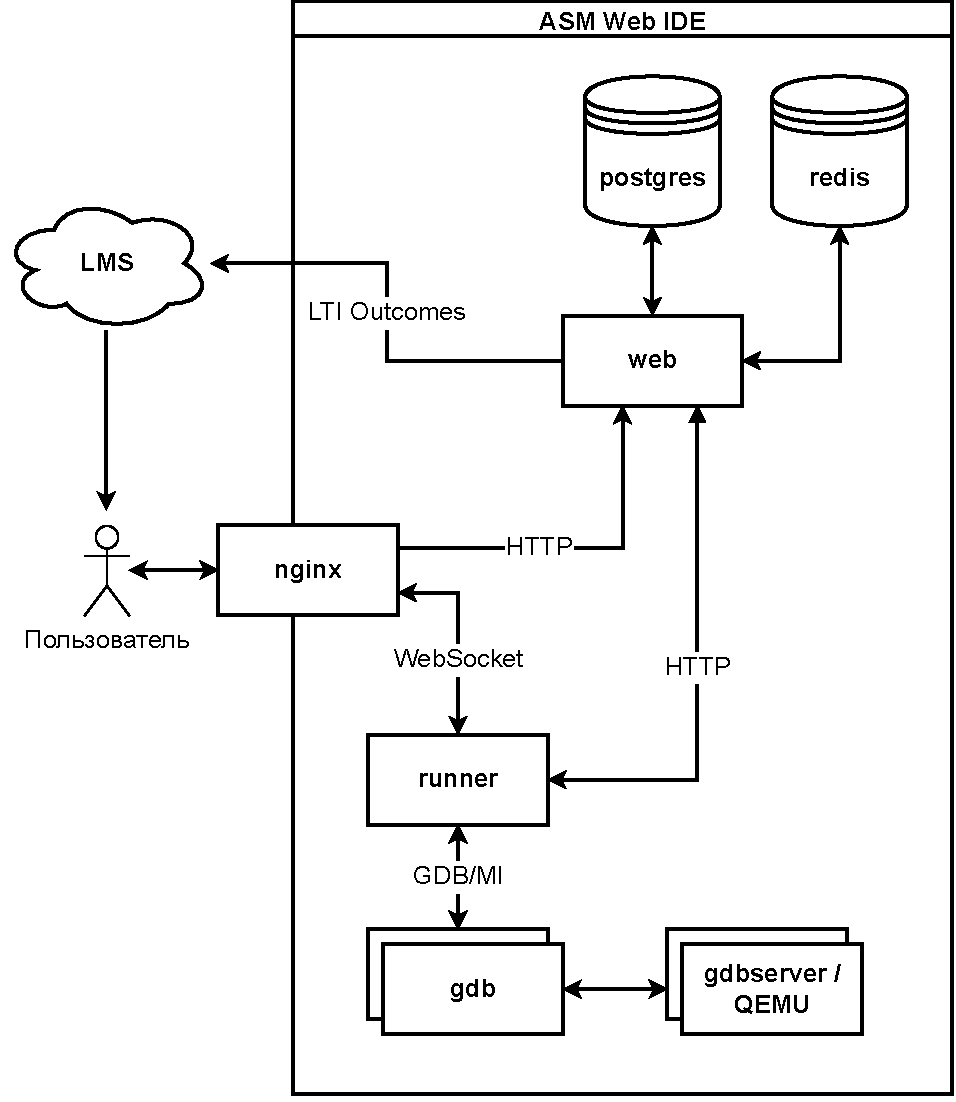
\includegraphics{images/processes_arch.pdf}}
        \caption{\label{fig:processes_arch} Схема взаимодействия процессов в системе}
    \end{center}
\end{figure}

Сервис \textbf{web} отвечает за основную бизнес-логику инструмента. Сервис предоставляет функционал аутентификации и авторизации, как через протокол LTI, так и по паре логин/пароль. Для студентов сервис предоставляет интерфейс просмотра задач и отправки решений, а для преподавателей~--- панель управления, позволяющую создавать и редактировать задачи, просматривать попытки решения и информацию о пользователях.

Сервис \textbf{runner} отвечает за управление сессиями отладки, взаимодействие с процессами отладчика через протокол GDB/MI, а также за взаимодействие с пользователями через протокол WebSocket. Помимо предоставления возможности интерактивной отладки веб-интерфейсу, этот сервис также занимается автоматизированной проверкой решений. Эта функциональность недоступна для внешнего пользователя напрямую, запросы на проверку решений отправляет сервис web по протоколу HTTP.

Базы данных \textbf{postgres} и \textbf{redis} используются для хранения необходимой для работы системы информации. В PostgreSQL хранится информация о пользователях, задачах, заданиях и посылках. Также там хранится метаинформация об интерактивных сессиях отладки. В Redis хранится множество использованных значений nonce при авторизации систем управления обучением по протоколу LTI.

Веб-сервер \textbf{nginx} используется в качестве обратного прокси-сервера, проксирующего HTTP запросы в сервис web и взаимодействие по протоколу WebSocket с сервисом runner. Также Nginx отдаёт статические файлы, необходимые для работы с веб-сервисом, такие как Javascript скрипты и файлы CSS.

\subsection{Модель данных}

Разрабатываемая система в своей работе оперирует различными сущностями. В этом разделе приводится описание этих сущностей и их взаимодействия между собой.

Для своей работы, система должна иметь доступ к основной информации о системах управления обучением, с которыми она взаимодействует. Эта информация представляется в виде сущности под названием tool consumer (потребитель инструмента), так как именно такое название используется в описании протокола LTI\cite{lti}. Сама система, в свою очередь, выполняет роль tool provider (поставщик инструмента). Протокол LTI описывает, как потребители и поставщики инструментов взаимодействуют. Для взаимодействия между собой, обоим сторонам нужно знать общий ключ и секретную строку.

Система также оперирует пользователями и сохраняет определённую информацию о них. К такой информации относится, например, почтовый адрес, полное имя пользователя и метод входа в систему: через привязку к определённому потребителю инструмента, или через предоставление имени пользователя и пароля. Также, система различает привилегированных и непривилегированных пользователей. Привилегерованные пользователи имеют доступ ко всем сущностям системы, а также могут добавлять и удалять интеграции с внешними системами управления обучением.

Ещё одной сущностью, которая необходима для работы системы, является задача. Задачи привязываются к конкретному потребителю инструмента при первом запуске (LTI launch \cite{lti}). Система сохраняет различную информацию о задаче, такую как её название, её условие, а также информацию, необходимую для проверки решений по этой задаче. К такой информации относится, например, архитектура ассемблера, используемая для решений этой задачи, алгоритм проверки решений и его параметры. Для переиспользования схожих алгоритмов проверки решений между различными задачами, такие алгоритмы вынесены в отдельный класс сущностей под названием checker (проверяющая программа).

В рамках разрабатываемой системы, такие проверяющие программы пишутся на языке Python и используют специальную библиотеку, предоставляющую доступ к многим часто используемым функциям. В свою очередь, это позволяет избавиться от необходимости формулировать задачи как набор тестов, которые подаются программе на стандартный поток ввода, а затем её вывод сравнивается с эталонным ответом. Также, такой подход позволяет выполнять проверку решений на архитектурах, не имеющих системных вызовов для вывода данных в стандартный поток вывода, например на микроконтроллерах без какой-либо операционной системы и периферии.

Информация о связи конкретного пользователя с конкретной задачей содержится в сущности <<задание>>. К этой информации относится время начала выполнения задания, оценка, информация, необходимая для отправки результатов проверки потребителю инструмента через протокол LTI Basic Outcomes, а также информация о правах пользователя по отношению к этой задаче. Пользователь может быть как студентом, так и преподавателем, при этом преподаватель не обязательно является администратором всей системы. Это позволяет разграничивать доступ к различным задачам для разных пользователей. Права конкретного пользователя передаются потребителем инструмента в авторизованном сообщении LTI launch \cite{lti}.

При отправке решения на проверку, система сохраняет информацию о посылке. К такой информации относится, например, исходный код, время посылки, оценка и комментарий проверяющей программы. Оценка за задание выставляется как максимум из оценок за все посылки этого пользователя по данной задаче.

Также система работает с сессиями отладки. При запуске программы в интерактивном отладчике, создаётся сессия отладки, которая привязана к конкретному пользователю и задаче. Общая информация о прошедших сессиях отладки сохраняется в базе данных. К этой информации относится запускаемый исходный код, архитектура процессора, время запуска и завершения сессии, а также объём потреблённых ресурсов: астрономического и процессорного времени, а также объём использованной оперативной памяти.

\subsection{Архитектура сервиса runner}

Сервис runner представляет из себя приложение, написанное на языке Python с использованием библиотек AsyncIO и AIOHTTP. Выбор данных библиотек обусловлен необходимостью асинхронного взаимодействия, как с пользователем, так и с запускаемыми программами.

\subsubsection{Структура классов}

Схема основных классов в сервисе представлена на рисунке \ref{fig:runner_classes}.

\begin{figure}[ht]
    \begin{center}
        \scalebox{0.8}{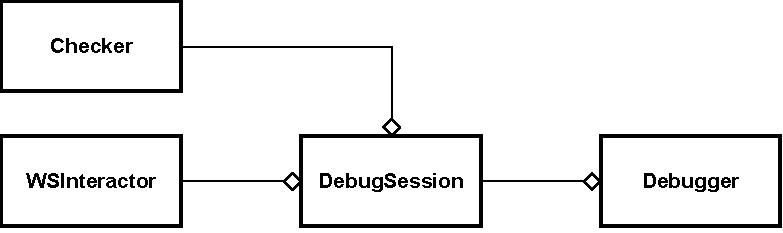
\includegraphics{images/runner_classes.pdf}}
        \caption{\label{fig:runner_classes} Схема основных классов сервиса runner}
    \end{center}
\end{figure}

Объекты этих классов отвечают за ресурсы, которыми они непосредственно управляют, а также за ресурсы вложенных классов. Для освобождения ресурсов принята конвенция: каждый из этих классов предоставляет метод \texttt{close()}, освобождающий ресурсы объекта, на котором он был вызван, а также вызывающий такой же метод на вложенных объектах. Это позволяет использовать функцию \texttt{contextlib.closing} для построения контекстов оператора \texttt{with}. Управление ресурсами в программах на языке Python через использование подобных менеджеров контекстов является хорошей практикой, потому что гарантирует детерминированную сборку ресурсов, даже при наличии исключений \cite{fluentpython}.

Класс \texttt{Debugger} отвечает за взаимодействие с процессом отладчика GDB. Он абстрагирует внутри себя запуск GDB, а также отправку ему команд и получение ответов от него.

Класс \texttt{DebugSession} включает в себя как поле объект класса \texttt{Debugger}. Сам этот класс отвечает за сессию отладки: компиляцию и запуск самой отлаживаемой программы, а также предоставляет интерфейс для взаимодействия с ней, например методы чтения и записи в регистры и память, а также методы для работы с точками останова, управления пошаговым исполнением и получении информации о использованных ресурсах. Эти методы формируют команды отладчику, исполняют их и преобразуют ответы в удобный для потребителя вид.

Класс \texttt{WSInteractor} отвечает за взаимодействие с пользователем интерактивного окна отладки по протоколу WebSocket. Протокол WebSocket позволяет передавать UTF-8 строки \cite{websocketrfc}, \texttt{WSInteractor} общается с клиентом, передавая JSON объекты, сериализованные в такие строки. Такие объекты могут содержать команды от пользователя или информацию о статусе запущенной программы. Таким образом, данный класс служит адаптером для взаимодействия с сессией отладки по протоколу WebSocket.

Класс \texttt{Checker} является родительским классом для разработки проверяющих программ. При проверки решения студента, создаётся объект дочернего класса \texttt{Checker}, соответствующий нужной проверяющей программе. Сама такая программа использует интерфейс класса \texttt{DebugSession} для выполнения различных действий над программой студента. Например, проверяющая программа может записать какой-либо объект в память, выполнить функцию, а затем сверить значение в регистре проверяемой программы с нужным.

\subsubsection{Компиляция ассемблерных программ}

В качестве компилятора система использует GCC. GCC (GNU Compiler Collection) представляет собой набор компиляторов для различных языков программирования, в том числе и для ассемблера. GCC позволяет генерировать машинный код на самые разные архитектуры, включая нужные нам x86-64 и AVR \cite{gcc}. Для архитектур x86 и x86-64 поддерживаются два диалекта ассемблера: AT\&T и Intel.

При составлении задач часто бывает так, что перед прроверкой решения необходимо добавлять программный код к началу или концу решения учащегося. Это вызывает несоответствие номеров строчек в коде и сообщениях об ошибках. GCC позволяет использовать в ассемблерном коде директиву \texttt{\#line} для перенумерации строк.

Компиляция ассемблерных программ для архитектуры x86-64 производится с использованием следующих аргументов компилятора:

\begin{enumerate}
    \item \texttt{-nodefaultlibs}. Данный параметр выключает связывание с библиотеками по умолчанию, необходимых в программах на языках C и C++, но не нужных для решения тех задач на языке ассемблера, для которых предназначается данная система.
    \item \texttt{-nostartfiles}. Этот параметр выключает связывание с объектным файлом \texttt{crt0.o}. Так как связывание со стандартной библиотекой языка C выключено, попытка связывания с этим объектным файлом окончится неудачей.
    \item \texttt{-static}. Этот параметр включает режим статического связывания. Так как программа не использует никаких разделяемых библиотек, данный флаг помогает уменьшить размер исполняемого файла и время компиляции.
    \item \texttt{-g}. Данный параметр включает добавление отладочной информации в результирующий двоичный файл. Отладочная информация необходима для просмотра текущей строки в режиме интерактивной отладки.
\end{enumerate}

В свою очередь, компиляция ассемблерных программ для архитектуры AVR производится с использованием других аргументов компилятора. Это обусловлено тем, что в архитектуре AVR нет такого понятия, как разделяемая библиотека, а также тем, что нет необходимости запрещать доступ к определённым системным вызовам, так как весь код запускается внутри эмулятора. Параметры компилятора приведены ниже:

\begin{enumerate}
    \item \texttt{-mmcu=atmega328p}. Данный параметр выбирает целевой микроконтроллер. В качестве такого микроконтроллера, был выбран Atmel ATmega328P из-за своей популярности, связанной с его использованием в одноплатном компьютере Arduino UNO \cite{arduinouno}.
    \item \texttt{-g}. Как и в случае с x86-64, данный параметр включает добавление отладочной информации в результирующий двоичный файл.
\end{enumerate}

\subsubsection{Изоляция ассемблерных программ}

Сервис runner использует несколько механизмов для обеспечения изоляции и ограничения потребляемых ресурсов пользовательскими программами.

Для запуска пользовательских программ используются Docker контейнеры. Docker позволяет ограничивать использование процессорного времени и используемую память в контейнерах через механизмы контрольных групп \cite{dockerlimits}. Общее используемое процессорное время можно ограничить системным вызовом \texttt{setrlimit}, используя параметр \texttt{RLIM\_CPU} \cite{setrlimit}. Docker позволяет это делать через параметр \texttt{ulimit} в командах запуска контейнеров. Создание и управление Docker-контейнерами производится через Docker Engine API. Данное API предоставляет REST-подобный HTTP-интерфейс для управления контейнерами.

Также, Docker позволяет изолировать программы по сети, ограничивать размер дискового пространства и накладывать другие ограничения на запускаемую программу. Но даже при запуске программы с минимальными привелегиями в изолированном по сети, процессорному времени, памяти и диску контейнере, программа может совершать нежелательные действия. К таким действиям, например, можно отнести использование системного вызова \texttt{ptrace}, позволяющего определять и запрещать подключение отладчика к программе.

Поэтому, для программ архитектуры x86-64 используется только изоляция по памяти и процессорному времени. Для всех остальных нежелательных системных вызовов, сервис runner использует \texttt{seccomp}~--- механизм ядра Linux, позволяющий процессу перейти в <<безопасный режим>>, в котором запрещены все системные вызовы, кроме \texttt{exit}, \texttt{sigreturn}, \texttt{read} и \texttt{write} \cite{seccomp}. Запретить работать со стандартными потоками ввода/вывода можно, вызвав \texttt{close} на них перед переходом в безопасный режим.

Ниже приведён исходный код, переводящий программу на языке ассемблера x86-64 в безопасный режим, предварительно закрыв стандартные потоки ввода, вывода и ошибок.

\begin{minted}{gas}
_start_seccomp:
    mov $3, %rax        # SYS_close
    mov $0, %rdi        # STDIN_FILENO
    syscall

    mov $3, %rax        # SYS_close
    mov $1, %rdi        # STDOUT_FILENO
    syscall

    mov $3, %rax        # SYS_close
    mov $2, %rdi        # STDERR_FILENO
    syscall

    mov $157, %rax      # SYS_prctl
    mov $22, %rdi       # PR_SET_SECCOMP
    mov $1, %rsi        # SECCOMP_MODE_STRICT
    syscall

    xor %rax, %rax
    xor %rdi, %rdi
    xor %rsi, %rsi
    jmp _start
\end{minted}

При использовании архитектуры AVR, запуск ассемблерных программ происходит с помощью эмулятора QEMU. Помимо прочего, QEMU позволяет запускать образы программ для микроконтроллеров на основе семейства архитектур AVR в режиме полносистемной эмуляции. В этом случае, процесс QEMU изолируется через Docker, аналогично случаю запуска кода x86-64 без использования эмулятора.

\subsubsection{Отладка ассемблерных программ}

Для запуска пользовательского кода в режиме отладки используется GDB. GDB (GNU Debugger) представляет из себя консольный инструмент отладки программ. GDB Позволяет отлаживать программы на самых разных языках программирования на разных платформах \cite{gdb}. Также инструмент поддерживает отладочную информацию в формате DWARF, что позволяет, например, узнавать, на какой конкретно строке исходного кода находится сейчас исполнение.

GDB/MI (GDB Machine Interface, машинный интерфейс GDB)~--- это один из форматов взаимодействия с GDB. В то время, как формат взаимодействия по умолчанию ориентирован на интерактивные терминальные сенасы, GDB/MI предназначен в первую очередь для использования другими программами, в которых отладчик является лишь одним компонентом целой системы.

При запуске программы под архитектурой x86-64, сервис runner создаёт Docker-контейнер для целей изоляции и запускает в нём утилиту под названием GDB server. Эта утилита предоставляет <<мост>> для GDB для отладки программы внутри запущенного контейнера. Это позволяет не ограничивать сам процесс GDB в ресурсах вместе с запускаемой программой. GDB server общается в GDB по протоколу TCP внутри одного физического хоста, но между разными контейнерами.

Так как GDB server работает только для родной архитектуры машины, на которой он запускается, при запуске ассемблерных программ с использованием эмуляторов, необходим другой механизм взаимодействия с GDB. Для этих целей, QEMU предоставляет свой собственный сервер, реализующий протокол GDB под названием GDB stub \cite{gdbstub}. В отличие от GDB server, он не реализует некоторые полезные расширения протокола взаимодействия GDB Remote Serial Protocol, такие как передача файлов и перезапуск программы. Поэтому, при запуске программ на архитектуре AVR, для их перезапуска используется установка регистра PC в значение 0. Для микроконтроллера ATmega328P это соответствует вызову обработчика прерывания RESET, который вызывается при перезагрузке или включении микроконтроллера \cite{atmega328p}.

\subsection{Архитектура сервиса web}

Сервис web представляет из себя приложение, написанное на языке Python с использованием фреймворка Flask. Выбор фреймворка обусловлен тем, что для Flask существует большое количество различных расширений, которые упрощают разработку веб-приложений. В разрабатываемой системе используется несколько таких расширений.

\subsubsection{Взаимодействие по протоколу LTI}

Для взаимодействия с обучающими системами по протоколу LTI используется библиотека \texttt{lti}. Данная библиотека предоставляет утилиты для разбора подписанных согласно протокоул OAuth сообщений в формате LTI, а также механизмы отправки таких сообщений \cite{pythonlti}.

\begin{figure}[ht]
    \centering
    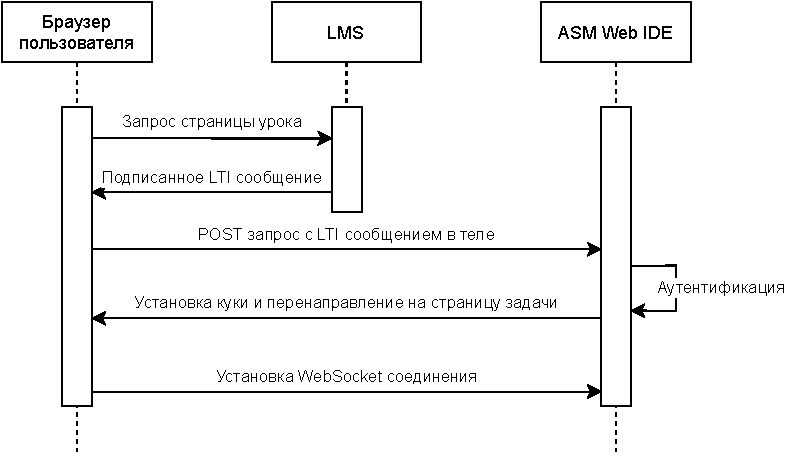
\includegraphics{images/lti.pdf}
    \caption{Диаграма запуска инструмента через LTI интеграцию}
    \label{fig:lti_diagram}
\end{figure}

На рисунке \ref{fig:lti_diagram} показана диаграма взаимодействия браузера пользоватееля, обучающей системы и разрабатываемого инструмента при открытии студентом задания. При запросе страницы урока, система управления обучением создаёт специальное сообщение, подписанное согласно протоколу OAuth 1.0 \cite{lti}. Данное сообщение содержит большое количество различных параметров, ниже приводится описание тех, которые используются в разрабатываемом инструменте

\begin{enumerate}
    \item \texttt{oauth\_version}. Данное поле содержит версию протоколу OAuth. Согласно спецификации LTI 1.1, данное поле всегда должно иметь значение \texttt{1.0}.
    \item \texttt{oauth\_nonce} и \texttt{oauth\_timestamp}. Данные поля используются для защиты от повторных отправок одного и того же сообщения. В поле \texttt{oauth\_timestamp} должна содержаться метка Unix-времени отправки запроса. Это время не должно отличаться от системного времени сервера больше, чем на десять минут.
    \item \texttt{oauth\_consumer\_key}, \texttt{oauth\_signature} и \texttt{oauth\_signature\_method}. Данные поля предоставляют возможность аутентифицировать автора LTI сообщения, как конкретную систему управления обучением, а также убедиться в целостности этого сообщения.
    \item \texttt{user\_id}. Данное поле содержит уникальный идентификатор пользователя в системе управления обучением. Если в базе данных инструмента ещё нет информации об этом пользователе, то она создаётся и привязывается к нужной LMS.
    \item \texttt{lis\_person\_contact\_email\_primary} и \texttt{lis\_person\_name\_full}. Данные поля содержат персональную информацию о пользователе: его адрес электронной почты и полное имя соотвественно. Согласно спецификации, отсутствие этих полей означает то, что эти данные скрыты настройками приватности. Таким образом, даже если эти данные уже были сохранены в раньше, если при очередном запуске инструмента они не указаны, их требуется удалить из базы данных \cite{lti}.
    \item \texttt{context\_title} и \texttt{resource\_link\_title}. Значения этих полей используются в качестве названия курса и названия задачи по умолчанию.
    \item \texttt{lis\_result\_sourcedid} и \texttt{lis\_outcome\_service\_url}. Данные поля определяют, по какому адресу и идентификатору отправлять информацию о оценке решения студента. Эта информация передаётся по протоколу LTI Basic Outcomes \cite{ltioutcomes}.
    \item \texttt{roles}. Данное поле содержит разделённый запятыми список ролей пользователя относительно этой конкретной задачи. При наличии роли \texttt{Instructor}, инструмент предоставляет доступ к редактированию задачи, просмотру решений по ней и прочих привилегированных действия. При отсутствии такой роли в списке, считается что у пользователя нет никаких специальных прав касаемо этой задачи.
\end{enumerate}

\subsection{Интерфейс пользователя}

\subsubsection{Взаимодействие с интерактивным отладчиком}

Для интерактивной отладки необходимо не только передавать команды из веб-интерфейса в GDB, но и асинхронно реагировать на события, возникающие при отладки. К таким событиям, например, относится остановка программы на точке останова. К счастью, все современные браузеры поддерживают протокол WebSocket, который позволяет общаться клиенту и серверу полностью асинхронно, а не по модели запрос-ответ.

При установке соединения по протоколу WebSocket, браузер пользователя направляет запрос в сервис web, указывая при этом идентификатор задания. Сервис, в свою очередь, проверяет корректность данных и прав доступа, а затем возвращает перенаправление на закрытую конечную точку через заголовок \texttt{X-Accel-Redirect}. Nginx сконфигурирован так, что, видя такой заголовок от источника, он начинает перенаправлять весь последующий трафик в сервис runner. Весь последующий процесс интерактивной отладки происходит по протоколу WebSocket напрямую между браузером пользователя и сервисом runner.

Графический интерфейс интерактивной отладки позволяет ставить брейкпоинты, можно слать команды, можно смотреть на регистры, можно смотреть значения произвольных выражений. Обратите внимание на красивый редактор. Скриншот в paused состоянии.

\subsubsection{Интерфейс преподавателя}

Преподаватель создаёт задачу в LMS, может её редактировать, ура.

\subsubsection{Интерфейс администратора}

Позволяет просматривать пользователей, задачи, сессии отладки и настраивать LTI интеграцию, ура.

\subsection{Сбор метрик}

Поднимаем Prometheus, пишем туда нужные метрики. Идеи для релевантных метрик: задержка исполнения команд gdb, время реакции на команды пользователя, общее потребление памяти на процесс отладки (gdb + gdbserver + программа), потребление cpu на процесс отладки (интересует idle cpu usage).

\subsection{Запуск и развёртывание системы}

Используем Docker Compose. Для этого написан специальный скрипт \texttt{manage.py}, позволяющий удобно запускать и управлять запущенными микросервисами.

\pagebreak
\section{Исследование свойств решения}

\subsection{Измерение потребляемой памяти и процессорного времени}

Описываем, как собираем данные. По всей видимости cat изнутри контейнера. Измерить оверхед.

\subsection{Нагрузочное тестирование}

\pagebreak
\specialsection{Выводы}

Ну вот написали инструмент, все задачи поставленные во введении сделали.

\pagebreak
\begin{thebibliography}{1}
\printbibliography[heading=none]
\end{thebibliography}
\end{document}
